\documentclass{article}
\usepackage{lmodern, amssymb,amsmath, graphicx, hyperref}
% === bibliography package ===
\usepackage{natbib}
% \usepackage[colorinlistoftodos, prependcaption]{todonotes} % to use \todo 
\usepackage[margin=1in]{geometry}
\usepackage{csquotes}
\usepackage{setspace}
\hypersetup{
    colorlinks=true,
    linkcolor=blue,
    filecolor=magenta,      
    urlcolor=cyan,
    citecolor = black
}
\urlstyle{same}  % don't use monospace font for urls

  \title{Campaign Contributions and Bureaucratic Oversight: A Case Study of the Federal Energy Regulatory Commission}
    \author{Justin Grimmer\thanks{Professor, Stanford University} \and Devin Judge-Lord\thanks{Ph.D. Candidate, University of Wisconsin-Madison}\and Eleanor Neff Powell\thanks{Booth Fowler Associate Professor, University of Wisconsin-Madison}}
    \date{\today}
    
\graphicspath{{Figs/}}


\begin{document}

\maketitle
% \tableofcontents

% \bigskip
% \href{https://judgelord.github.io/correspondence/gh-pages/summary.html}{Project Summary} | 
% \href{https://docs.google.com/document/d/1fJxjXjAyRL9vX-16fSsH29anXZc-W74GMf_7BSgWkws/edit}{Codebook} |
% \bigskip

\begin{abstract}
\noindent 

In this paper we explore whether congressional letter-marking activity is driven by campaign contributions in the context of the Federal Energy Regulatory Commission.  Drawing on 10 years worth of letters from legislators to the commission, we find that these letters are filled with specific references to companies (and in some instances the CEOs) they are seeking to assist.  We  match these letters with campaign finance records to see whether Members' efforts are primarily concerned with their donors or their constituents.  
\end{abstract}

\newpage
\doublespacing
\section{Introduction}

Concern over the potential for campaign contributions to influence the policy-making process has been a central question in American politics over the last several decades.  Much of the academic study in this area has focused around whether campaign contributions influence legislators' roll call votes.  While these numerous studies have produced somewhat mixed results, on the whole the answer appears to be no: that most of the time campaign contributions don't influence how a member votes in the context of a roll call vote.  While the academic focus on roll call votes is perhaps not surprising given the availability of the data, this precise availability and visibility makes them a poor vehicle for those seeking to quietly influence the policy-making process who may not want to draw scrutiny from journalist or constituents. 

In comparison to the intensity academic scrutiny given to roll call votes, much less attention has been given to congressional letter-marking activity--when legislators write letters to bureaucratic agencies urging them toward or against some regulatory decision.\footnote{This has begun to change in the last few years with recent studies by  \citet{MillsKalafHuges2015,Ritchie2017,Lowande2018JOP,LowandeRitchieLauterbach2018}.}  While technically these letters are subject to federal open records act requirements that process is often slow and laborious, meaning that in practice these letters rarely see the light of day and are highly unlikely to draw public scrutiny.  Thus letter-marking may be a preferred vehicle for those seeking to quietly influence the policy-making process through campaign contributions.  In this paper, we deeply examine one agency -- the Federal Energy Regulatory Commission--and whether campaign contributions to legislators appears to explain whether or not those legislators write letters to the agency on behalf of those companies.  


\section{Arnold's Impact: Studying Congress-Bureaucracy}

\section{Studying the Influence of Lobbying and Campaign Contributions on Congressional-Bureaucratic Relations}
\subsection{Findings: Previous Research on Influence of Money}
\subsection{How Corporations Can Make Political Contributions}

The campaign financing landscape has undergone substantial transformation over the last several decades. Perhaps the area of greatest change is the regulation surrounding how corporations (and other business entities) can engage in political activity.  As the Federal Election Commission's \textit{Campaign Guide for Corporations and Labor Unions} describes: \\ 

\singlespacing
\begin{quotation}
``The Federal Election Campaign Act (the Act) generally prohibits corporations ... from using their general treasury funds to make contributions to federal candidates, federal accounts of political party committees, and other political committees (PACS). 52 U.S.C. \S 30118(a). They may, however, fund independent expenditures, contribute to political committees established solely to finance independent expenditures (e.g., Super PACs), contribute to the non-contribution accounts of Hybrid PACs, and establish separate segregated funds (SSFs),"\citep[][pg.1]{FEC2018}.\footnote{Separate Segregated Funds (SSFs) are corporate sponsored political action committees \citep{FEC2018}.  The SSF may raise money in order to make contributions to and expenditures on behalf of federal candidates and committees.  The full name of the connected organization (sponsoring company or organization) must appear in the name of the SSF. The connected organization is the organization (corporation) that establishes, administers or financially supports the SSF.  The Connected Organization may exercise control over the SSF.  Note that if a connected organization has parent companies/subsidiaries those names don't need to be included in the name of the SSF. SSFs set up by parent/subsidiary corporations are automatically considered affiliates and bound by a single set of contribution limits.  SSF affiliates must be listed on its Statement of Organization.}
\end{quotation}

\doublespacing

\begin{table}
\caption{How Corporations Can Make Political Contributions}
\begin{center}
\begin{tabular}[ht!]{|l|p{5cm}|p{5cm}|}
\hline
& Method of Contribution & 2018 Rules \\
\hline
1. & Step 1: Company Contribution to Tax Exempt 501c. Step 2:  501c makes independent expenditures (advertising) & Varying amount of political activity by type of group.  501c(4) ``social welfare'' organizations can do unlimited amounts but must be less than 50\% of their total spending. \\ \hline
2. & Company Contribution to Separate Segregated Funds of PACs& \\  \hline
3. & Personal Contributions from Corporate Officers and Employees to Legislators& Limit of \$2700 per election (\$5400 for primary + general)\\  \hline
4. & Personal Contributions from Corporate Officers to PACs&\\  \hline
5. &Company contribution to Super PAC (independent expenditure only committee). Super PAC can make unlimited independent expenditures in support or opposition to legislator's election.& Company contributions to SuperPACs are unlimited. Independent Expenditures reported to FEC. Created post 2010 Speechnow.org vs. FEC ruling. Must disclose donors to FEC, can list corporations as donors and 501c nonprofits as donors (funders not disclosed to FEC).\\  \hline
6.&The corporation can directly make unlimited contributions to the non-contribution accounts of Hybrid PACs.  Hybrid PACs can make direct contributions to candidates, but also maintains a separate bank account to deposit/withdraw funds raised in unlimited amounts from corporations.   &The funds received from the corporations cannot be used to make direct or coordinated contributions to candidates but can be used for independent expenditures, which must be reported to the FEC.\\  \hline
7. & 527s Issue Advocacy& Prior to Citizen's United in 2010 couldn't advocate support or defeat of a candidate.\\  \hline
8.& Lobbyist Contributions from lobbyists that appear in the lobbying disclosure files.& \\ \hline
\hline
\end{tabular}
\end{center}
\end{table}


See: \citet{FEC2018}: \url{https://www.fec.gov/resources/cms-content/documents/colagui.pdf}
See: \url{https://bolderadvocacy.org/wp-content/uploads/2012/10/The_Connection_Ch4_paywall.pdf}

Note: Independent expenditures by federal contractors are prohibited.  
\section{Theory: What Motivates Legislator Lettermarking Activity}
\subsection{Theory: Influence of \$ on Lettermarking Activity}
\section{Letter-marking \& FOIA Data}

\subsection{Examples of FERC Letters}
\subsubsection{Example of Constituent Service Letter}
\clearpage
\subsubsection{Example of Personal Business Interest}

In some cases, legislators appeared motivated by personal business concerns.  For example, in 2014 former Florida Senator and Governor Bob Graham wrote to FERC regarding an issue that affected his family's farming business.\footnote{See  \url{http://miamilakes.com/AboutGraham/Overview.aspx} for a discussion of Senator Graham's relationship to the farm in question.}  

\begin{figure}[hbt!]
\centering
\caption{Example of Personal Business Interest} \label{f:examplepersonalbus}
\scalebox{0.8}{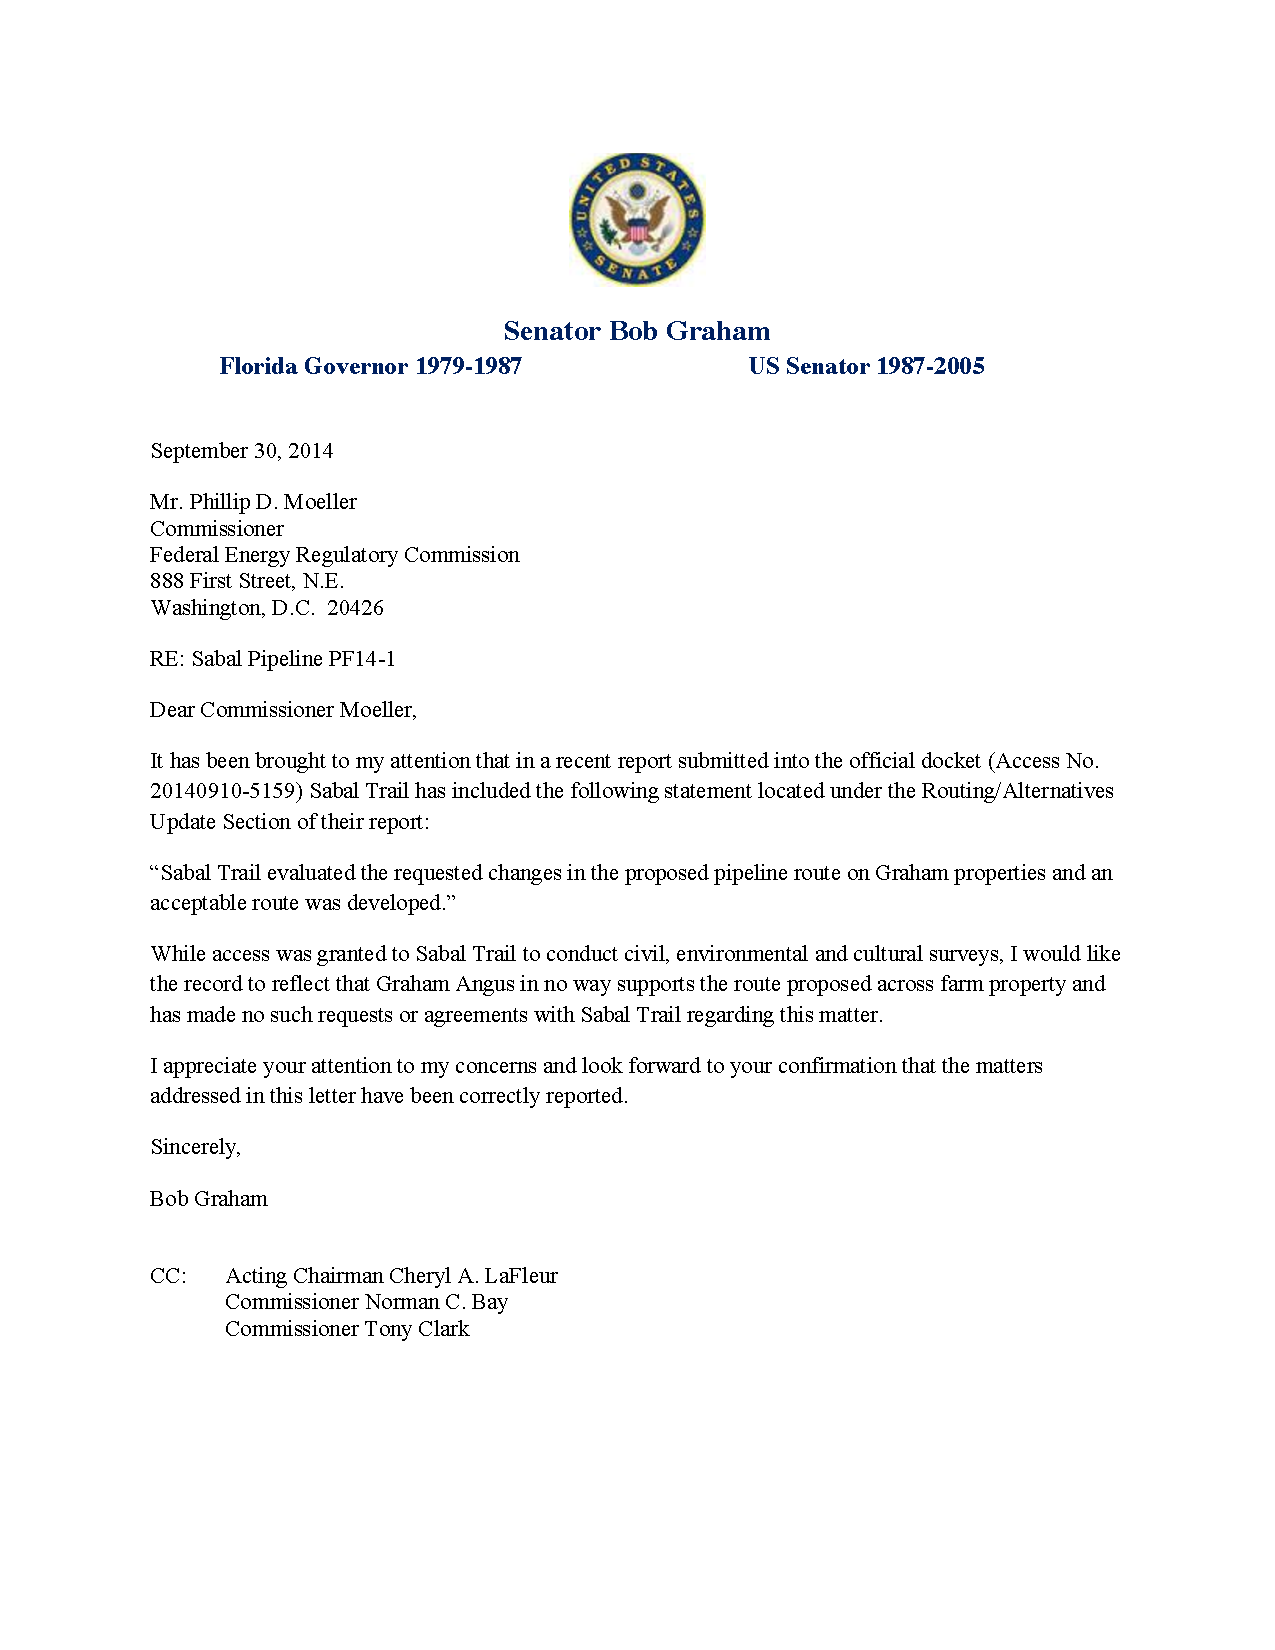
\includegraphics{20141002-4001-13649830small.pdf}}
\end{figure}


\section{Dependent Variable: Member Attempts to Influence Bureaucracy}

\section{Findings: Types of Congressional Requests to FERC}

\begin{figure}[hbt!]
\centering
\caption{Distribution Across Types of Congressional Requests to FERC 2000-2019} \label{f:fig2}
\scalebox{0.3}{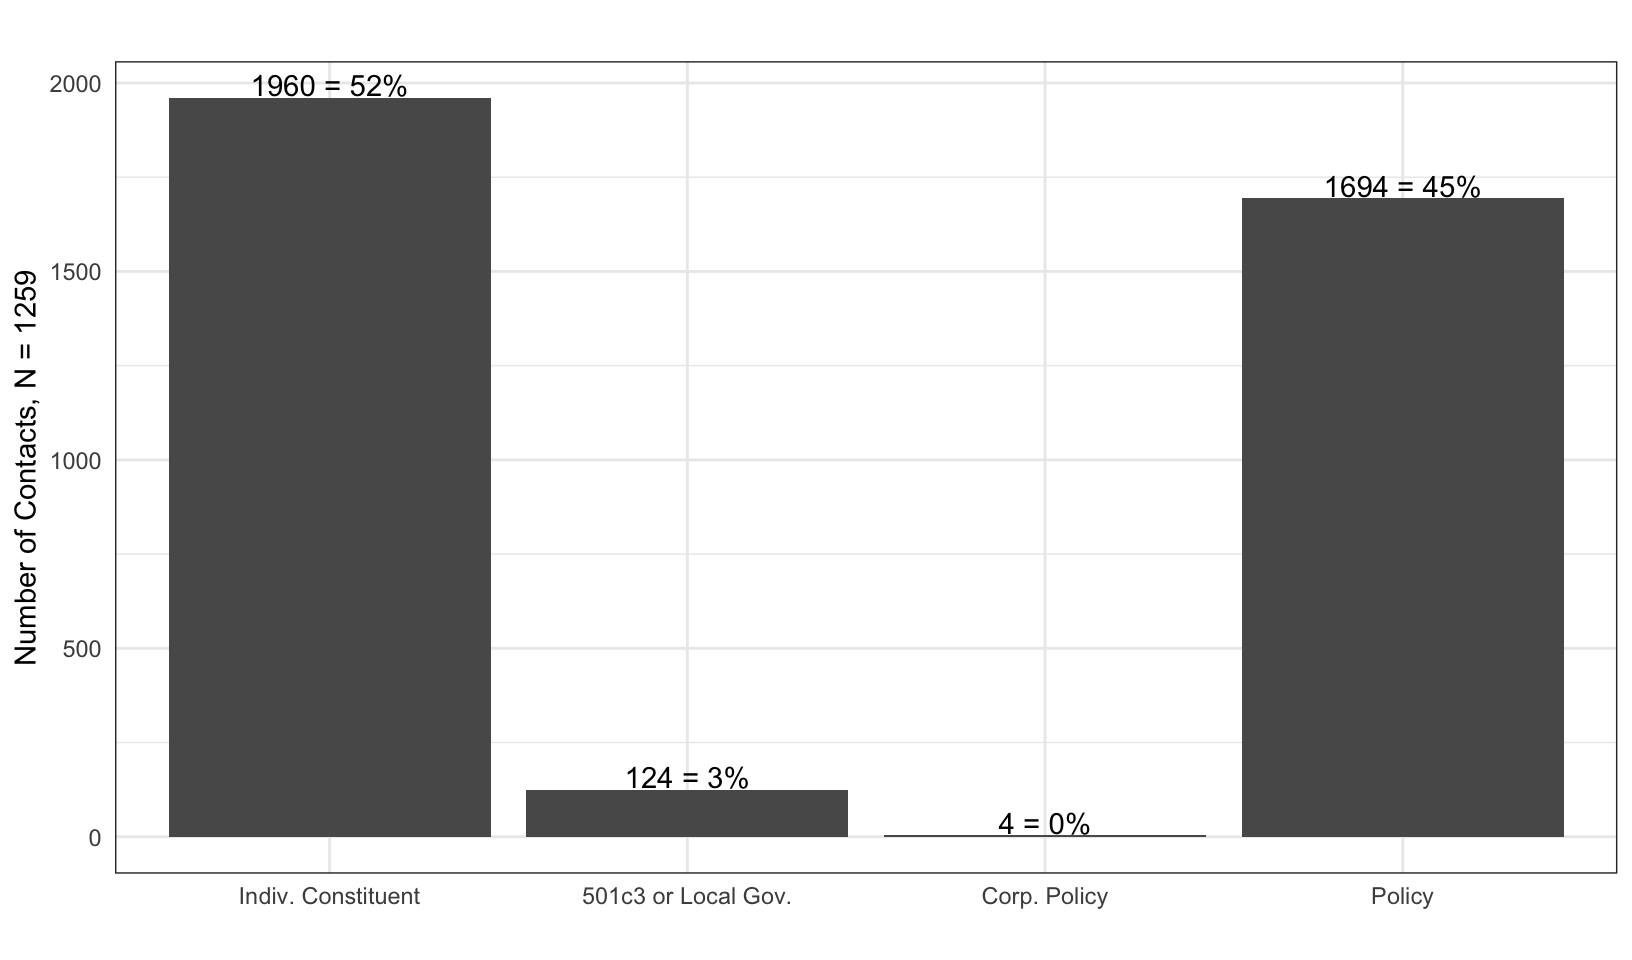
\includegraphics{data-coverage-by-type-1.png}}
\end{figure}

\clearpage
\section{Findings: What Members Attempt to Influence FERC}

In our research across federal agencies, we typically see senators from larger states doing more constituency service than senators from smaller states.  This isn't the case with letter-writing to FERC.  As figure \ref{f:statepop} below shows, letter-marking to the Federal Energy Regulatory Commission doesn't vary with state population.  

\begin{figure}[ht!]
\centering
\caption{State population and Attempts to Influence FERC}\label{f:statepop}

\includegraphics[width = \textwidth]{population-1}
\end{figure}

\begin{figure}[ht!]
\centering
\caption{Total Number of FERC Contacts from Senators by State}\label{f:statepoptotal}

\includegraphics[width = \textwidth]{sentate_percapita_map-1}
\end{figure}

\begin{figure}[ht!]
\centering
\caption{FERC Contacts Per Million Residents from Senators by State}\label{f:statepoppercap}

\includegraphics[width = \textwidth]{sentate_percapita_map-2}
\end{figure}




\begin{figure}[ht!]
\centering
\caption{Senators Most Attempting to Influence FERC}\label{f:senatebarcode}

\includegraphics[width = \textwidth]{members_barcoded-1}
\end{figure}

\begin{figure}[ht!]
\centering
\caption{Representatives Most Attempting to Influence FERC}\label{f:housebarcode}

\includegraphics[width = \textwidth]{members_barcoded-2}
\end{figure}



\clearpage

\subsection{Findings: Congressional Committee Chairs}

\begin{figure}[ht!]
\centering
\caption{House Committee Chairs Attempting to Influence FERC}\label{f:housechairs}
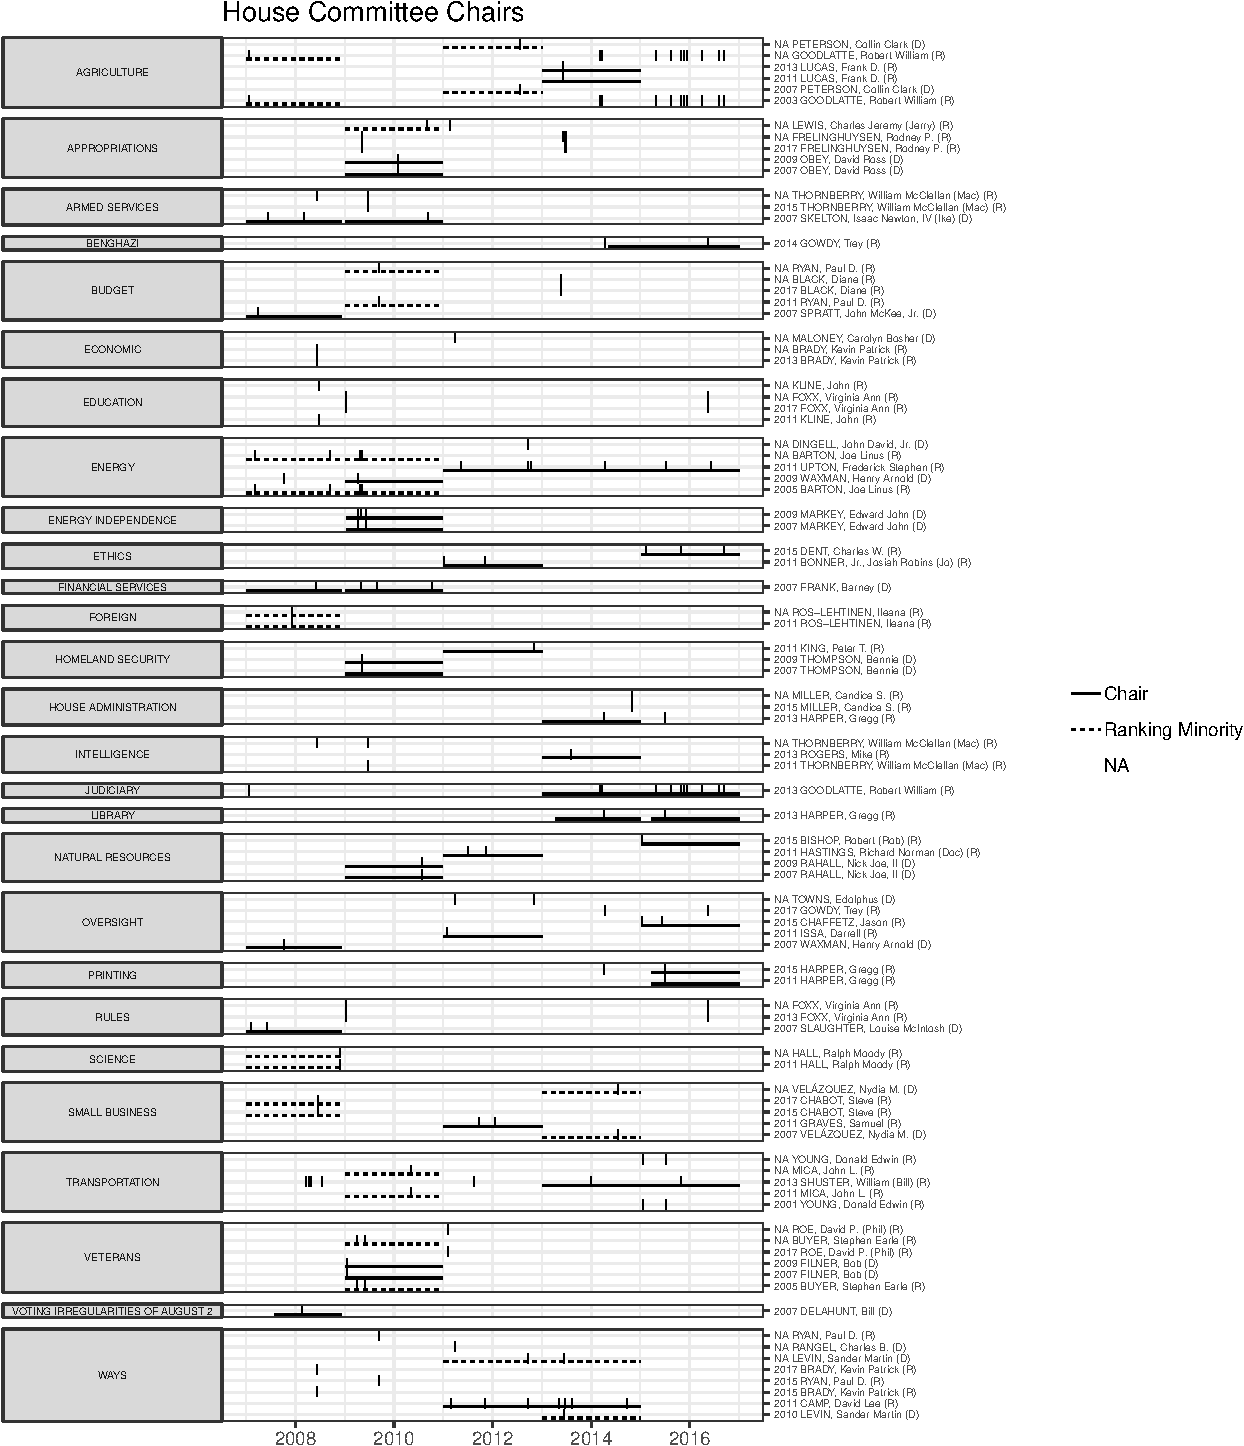
\includegraphics[width = \textwidth]{committeechiars_barcode_house-1}
\end{figure}

\begin{figure}[ht!]
\centering
\caption{Senate Committee Chairs Attempting to Influence FERC}\label{f:senatechairs}
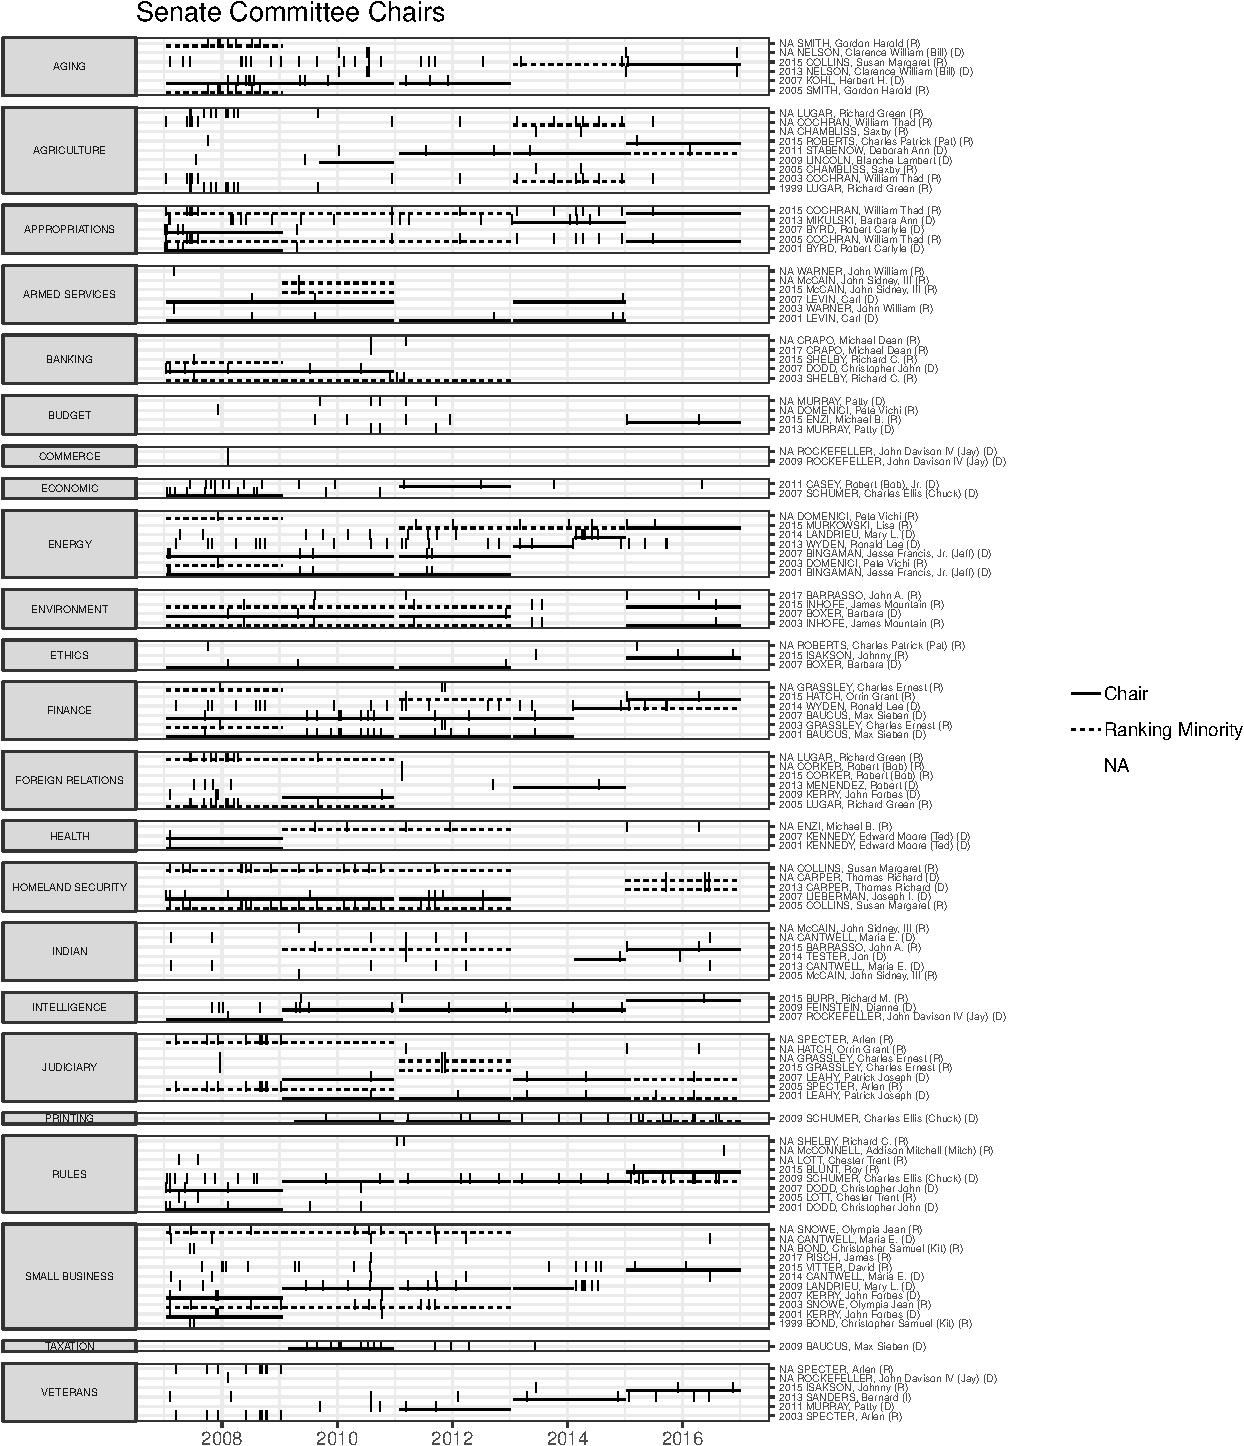
\includegraphics[width = \textwidth]{committeechiars_barcode_senate-1}
\end{figure}






\subsection{Findings: How do Attempts to Influence FERC Differ from other Lettermarking}
\section{Findings: What Members Attempt to Influence on Behalf of Constituents vs. Companies}
\section{Findings: How do Campaign Contributions Impact Member Lettermarking Activity}
\section{Conclusion}

\section{Future Research}
\begin{itemize}
\item Lobbying Data
\item Expansion to earlier time periods
\item Expansion to other agencies
\item Earmark Ban discontinuity
\item Speed of Review as an Outcome.  That's often what the companies are asking for in these requests.  
\end{itemize}

\bibliographystyle{chicago-apsr}

\bibliography{../congress2018.bib}
%\bibliography{congress2018}
%\newpage
%\listoftodos[Notes]


\end{document}
